
%{\normalfont\initfamily \fontsize{12mm}{12mm}\selectfont D}
\cappar Durante muitos anos foi possível constatarmos o enorme
interesse dos técnicos angolanos na sua formação. Tanto os que
estudaram dentro como os que tiveram a possibilidade de o fazer no
exterior, tiveram que realizar grandes esforços para conseguir
terminar os estudos devidos as dificuldades diversas quer seja de
ordem financeiras como de outras índoles próprias do tipo que durante
anos sofreram os que viveram a época penosa.

\begin{wrapfigure}{r}{0.35\textwidth} 
  \vspace{-25.5pt}
  \begin{figurebox}
    \vspace{20pt}
    \centering
    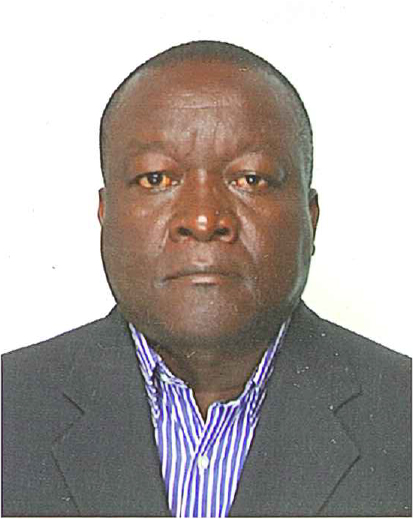
\includegraphics[height=0.28\textheight]{JoseManuelAlberto.jpg}\\
    José Manuel Alberto\\ 
    Diretor executivo\\
    {\sl SAEMA Projectos na área
      eléctrica e médica, LDA}
    %\vspace{0.1\textheight}
  \end{figurebox}
  \vspace{-10pt}
\end{wrapfigure}


Nasce essa revista com a vocação de dar um impulso e uma ajuda a estes
jovens e menos jovens técnicos e engenheiros que desejam fortalecer a
sua base de conhecimentos técnicos e científicos para poderem
participar em igualdade de condições com os milhares de técnicos que
desde fora acodem ao nosso país a participar na construção das suas
infraestruturas.  Os gregos diziam que o conhecimento se compõem de
teoria e praxis. É evidente que os técnicos angolanos dispõem de
suficiente praxis já que em poucas partes do mundo produziu-se tanto
como em Angola o que converteu o país num grande canteiro de obras.

Portanto é na teoria onde vamos fazer o encape especificamente nas
matemáticas como base de todo o conhecimento científico e técnico, com
o que iniciamos a aventura desta revista técnica SOLUÇÕES, fazendo uma
revisão a todas as ferramentas matemática que constituem a base do
nosso trabalho.

Para tudo isto contamos na nossa redação com gente altamente
especializada como Doutores em Ciências Exatas de renome para que nos
ponham ao dia nas mais importantes teorias dando-lhe sempre a
abordagem mais actual e utilizando também a ferramenta computacional
mais moderna que também vamos ter acesso.

Esperamos com esta revista SOLUÇÕES, poder munir os técnicos e
engenheiros do nosso país de conhecimentos fundamentais e
imprescindíveis para enfrentar os desafios sempre crescentes do
desenvolvimento tecnológico de um mundo moderno cada vez mais
exigente.


\vspace{20pt}

\begin{figurebox}
  \vspace{15pt}
  \centering
  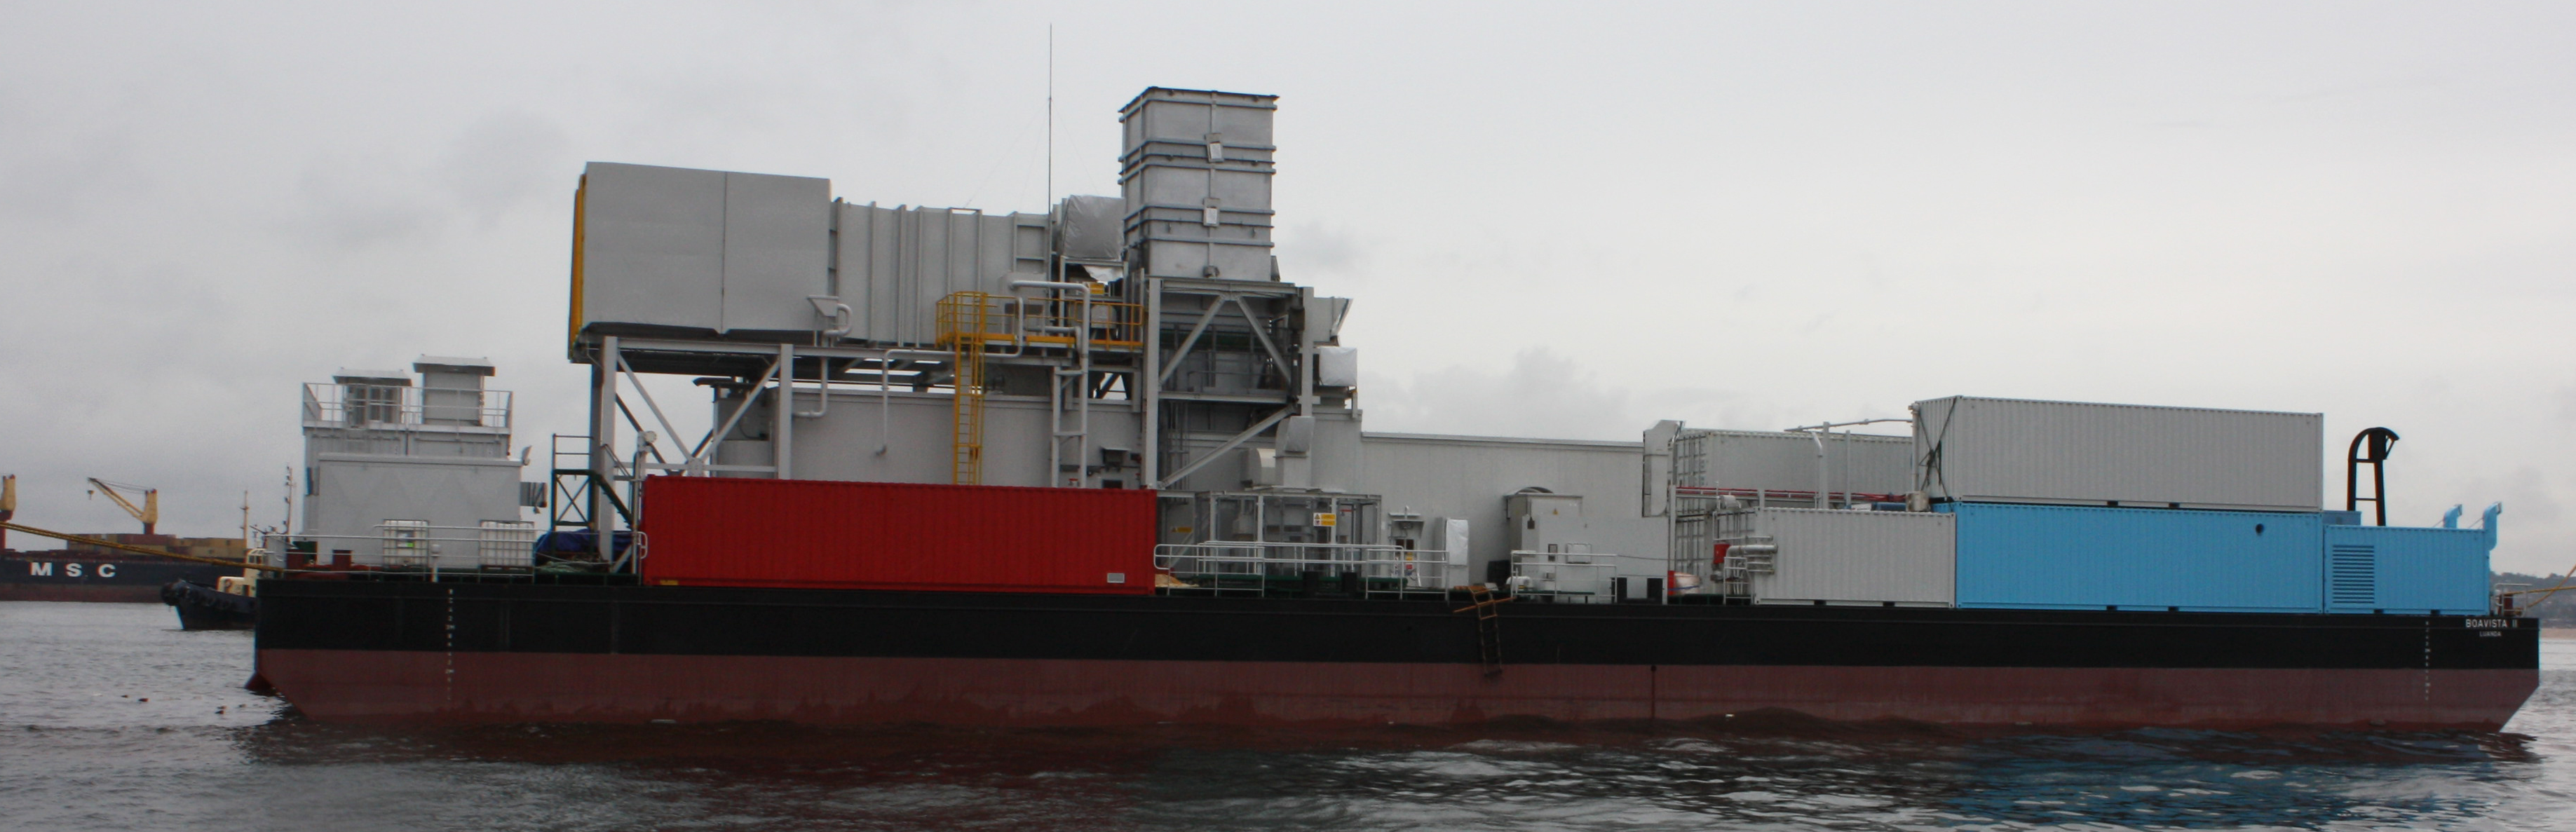
\includegraphics[width=0.9\textwidth]{barco.png}\\
  {Boavista II, central elétrica flutuante}
  \vspace{10pt}
\end{figurebox}

\newpage
%%% Local Variables: 
%%% mode: latex
%%% TeX-master: "nadaesimposible"
%%% End: 


